\mode*


\subsection{Notion d'asynchronisme}

\begin{frame}[fragile]{Un premier exemple}

    \begin{lstlisting}[numbers=none]
var t1 = new Thread(() -> {
  System.out.print("Hello ");
  System.out.print("World ");
});
var t2 = new Thread(() -> {
  System.out.print("Multithreaded ");
});
 
t1.start();
t2.start();

t1.join();
t2.join();

System.out.println("!");
    \end{lstlisting}
\vfill
\begin{block}{Expérience}
   \begin{itemize}
      \item Lancer le programme plusieurs fois. Qu'observe-t-on ? 
   \end{itemize}
\end{block}
\begin{citing}
\jitem \lstinline{cm2/HappensBefore.java}
\end{citing}
\end{frame}



%%%%%%%%%%%%%%%%%%%%%%%%%%%%%%%%%%%%%%%%%%%%%%%%%%%%%%%%%%%%%%%%%%%%%%%%% 

\begin{frame}[fragile]{Non déterminisme des sorties du programme}

    \begin{block}{Une exécution possible}
%    \begin{itemize}
%    \item  Toute action a un instant de début et un instant de fin
%    \end{itemize}
\scalebox{.7}{
      \begin{tikzpicture}
        \draw[alertColor,   -latex] (0,2) node[left]{$t1$}   +(3.4,0) -- (8.5,2);
        \draw[structure,    -latex] (0,1) node[left]{$main$}          -- (13.4,1);
        \draw[exampleColor, -latex] (0,0) node[left]{$t2$}   +(3,0) -- (8,0);
        \draw[->] (0,-.5) node[left]{temps réel}   -- (13.4,-.5);

        \draw[structure   , fill=structure!20, rounded corners]    (1.5 ,1)  +(-.8,-0.3) rectangle +(.8,0.3) +(0,0) node{$t1.start()$};
        \draw[structure   , fill=structure!20, rounded corners]    (3.2 ,1)  +(-.8,-0.3) rectangle +(.8,0.3) +(0,0) node{$t2.start()$};
        \draw[structure   , fill=structure!20, rounded corners]    (6.6 ,1)  +(-2.5,-0.3) rectangle +(2.5,0.3) +(0,0) node{$t1.join()$};
        \draw[structure   , fill=structure!20, rounded corners]    (10  ,1)  +(-.8,-0.3) rectangle +(.8,0.3) +(0,0) node{$t2.join()$};
        \draw[structure   , fill=structure!20, rounded corners]    (11.9,1)  +(-1,-0.3) rectangle +(1,0.3) +(0,0) node{$println(!)$};

        \draw[alertColor  , fill=alertColor!20, rounded corners]   (4.9 ,2)  +(-1,-0.3) rectangle +(1,0.3) +(0,0) node{$print(hello)$};
        \draw[alertColor  , fill=alertColor!20, rounded corners]   (7.0 ,2)  +(-1,-0.3) rectangle +(1,0.3) +(0,0) node{$print(world)$};
        \draw[exampleColor, fill=exampleColor!20, rounded corners] (5.5 ,0)  +(-2,-0.3) rectangle +(2,0.3) +(0,0) node{$print(multithreaded)$};

        \end{tikzpicture}
}
  \end{block}

  \begin{block}{Asynchronisme}
    Il est impossible de prévoir la vitesse d'exécution :
    \begin{itemize}
    \item  d'un thread par rapport à un autre,
    \item  d'une portion de code exécutée par un thread par rapport à une autre,
    \item  d'une exécution d'un thread par rapport à une autre.
    \end{itemize}
  \end{block}
  \begin{alertblock}{Question}
    \begin{itemize}
    \item Un programme n'est correct que si toutes ses exécutions le sont.
    \item Comment raisonner sur les exécutions concurrentes ?
    \end{itemize}
  \end{alertblock}
\end{frame}

\subsection{Relation happened before}

\begin{frame}{Causalité et concurrence}
  \vfill
  \begin{center}
     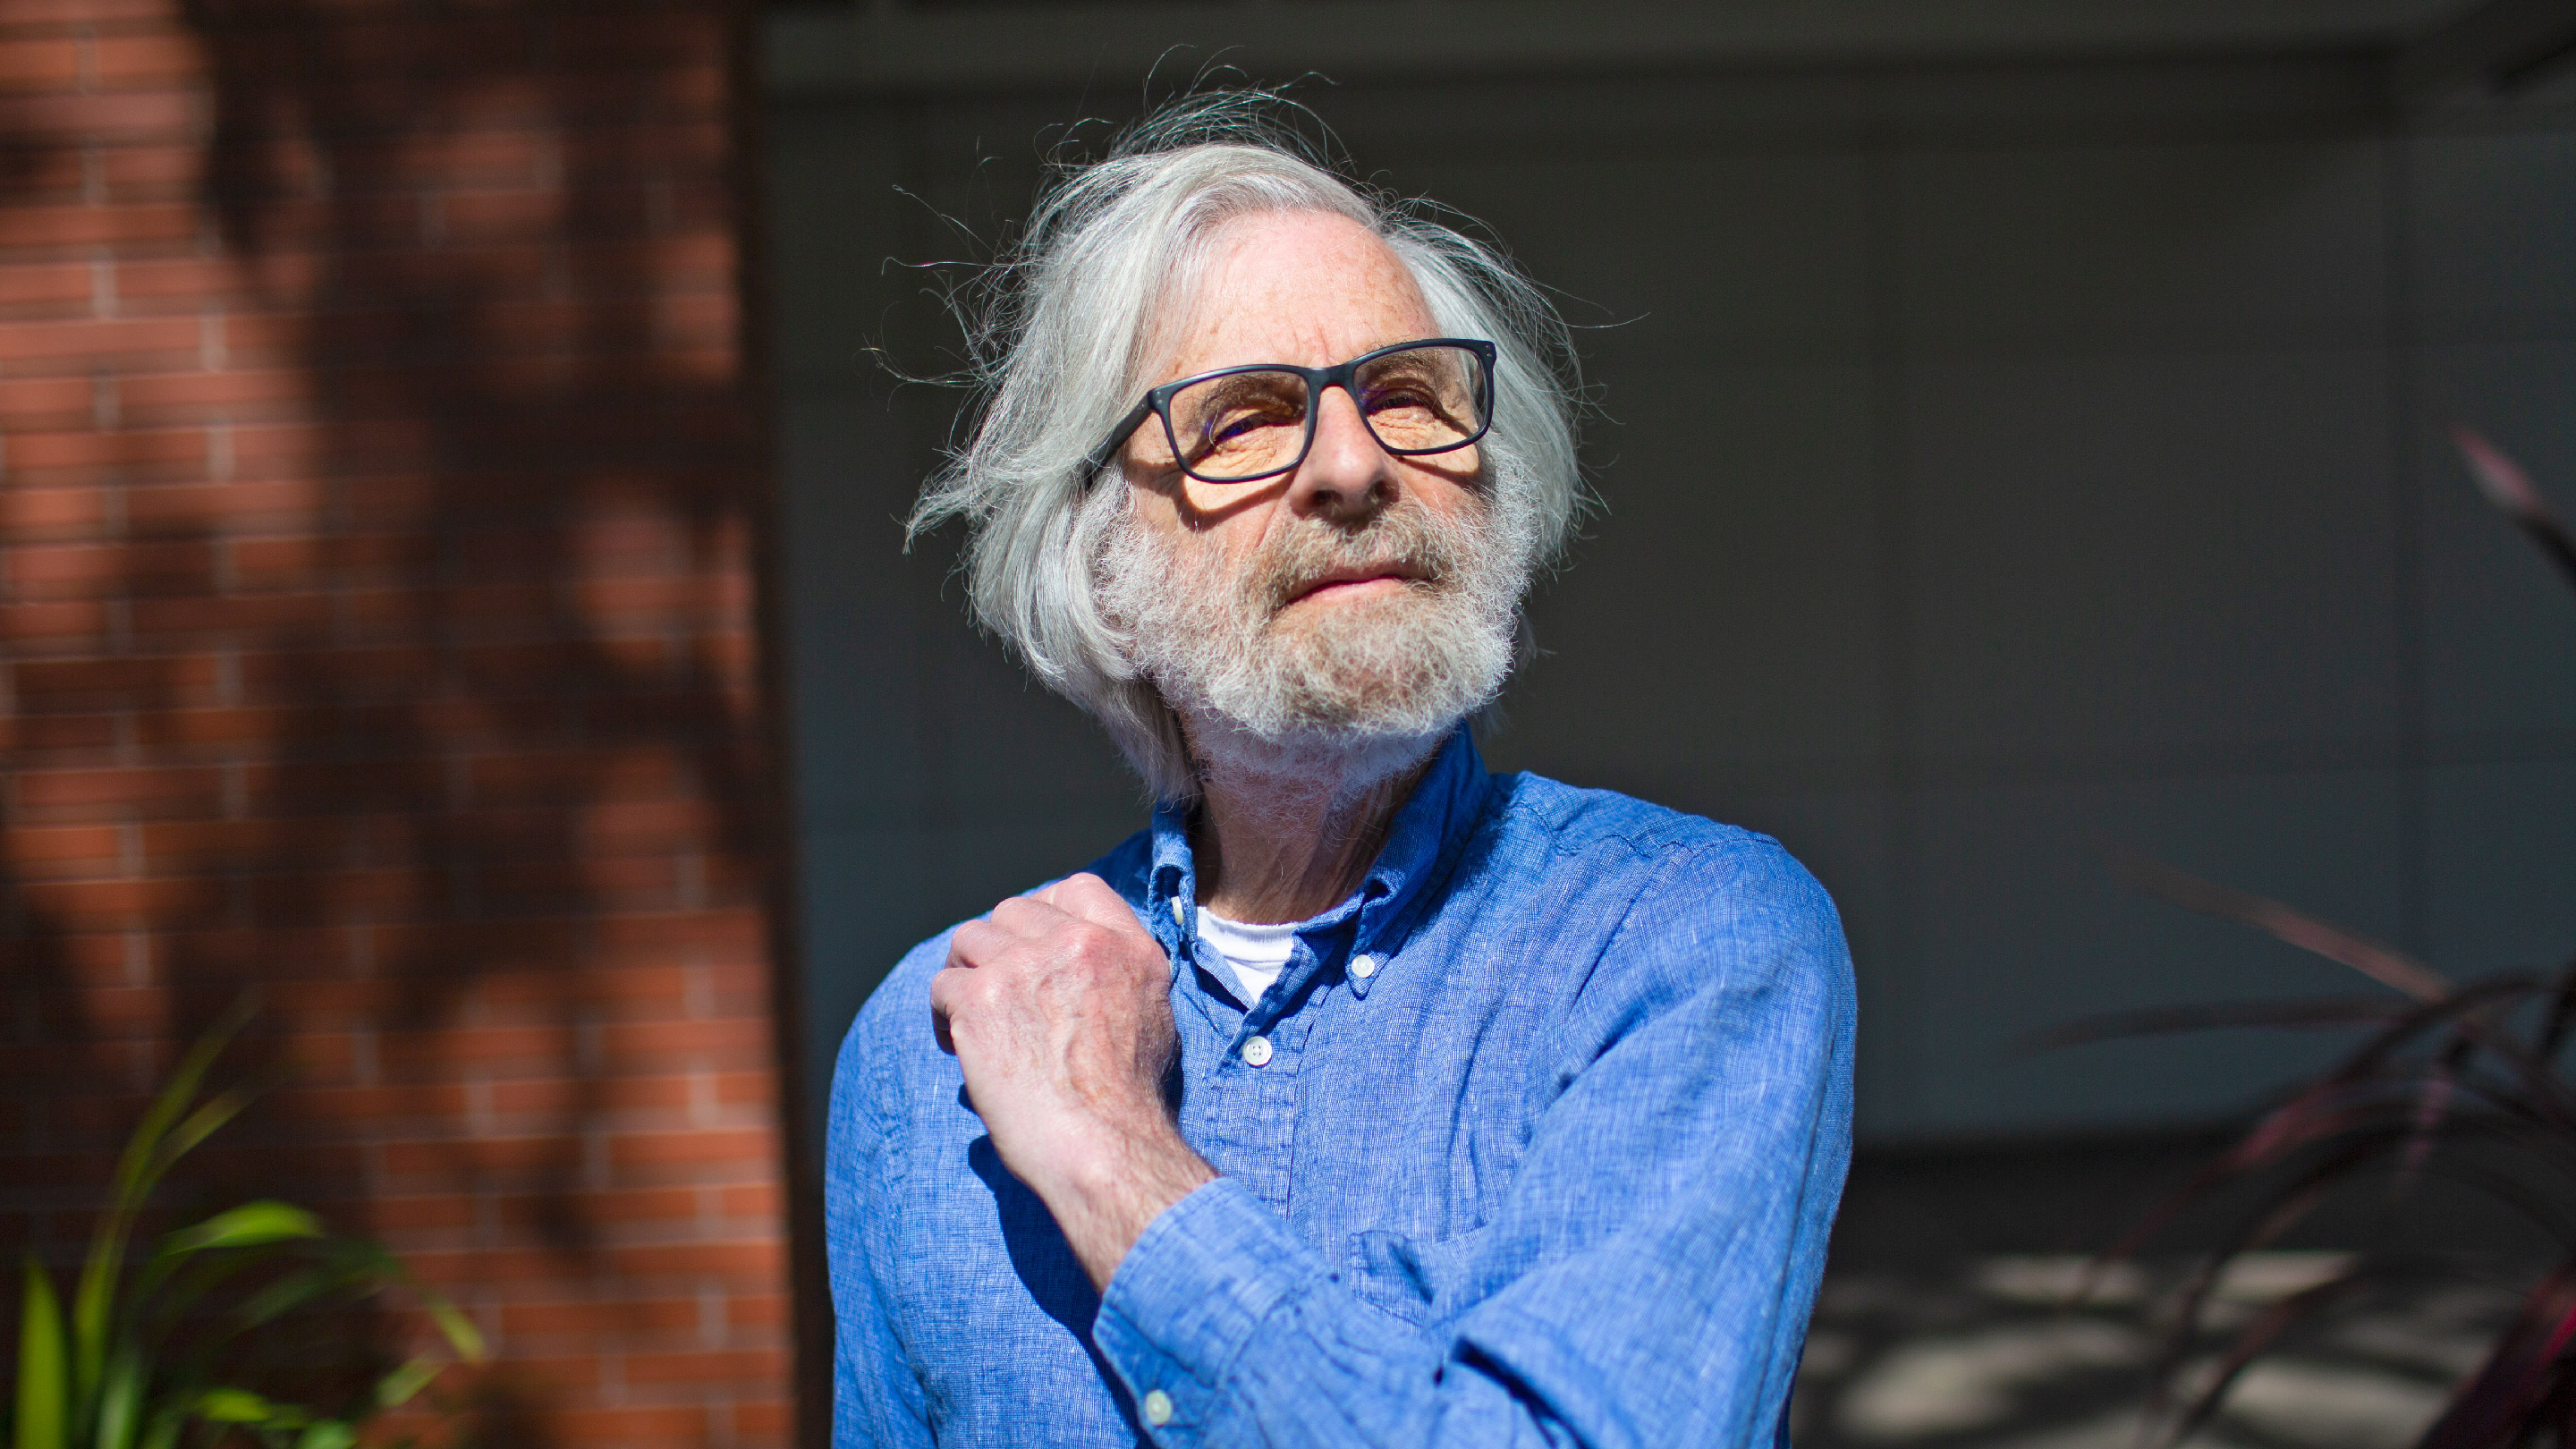
\includegraphics[height=5cm]{Lamport.jpg}\\
     Leslie Lamport\\
     Prix Turing 2013
  \end{center}
  \vfill
  \begin{citing}
  \item[L78] Leslie Lamport. \textit{Time, clocks, and the ordering of events in a distributed system.} CACM (1978)
  \item[L79] Leslie Lamport. \textit{How to make a multiprocessor computer that correctly executes multiprocess programs.} IEEE ToC (1979)
  \end{citing}
\end{frame}

\begin{frame}{La relation ``happened before'' (ordre causal)}
    \begin{shadequote}{Leslie Lamport}
    \small
    The \alert{concept of time} is fundamental to our way of
    thinking. \alert{It is derived} from the more basic concept of
    the \alert{order in which events occur}. (...)

    However, we will see that this concept must be carefully reexamined when considering events in a distributed system. (...)

    In a distributed system, it is sometimes impossible to
    say that one of two events occurred first. \alert{The relation
    "happened before" is therefore only a partial ordering
    of the events in the system.}
    \end{shadequote}

\begin{block}{Définitions}
    \begin{itemize}
    \item $e\mapsto e'$ si l'une des trois conditions s'applique :    
       \begin{itemize}
       \item \structure{Ordre de programme :} le même thread produit $e$ puis $e'$
       \item \structure{Précédence sémantique :} (précisé plus tard)
       \begin{itemize}
       \item Par exemple, $e = t.start()$ et $e'$ produit par $t$
       \item Par exemple, $e$ produit par $t$ et $e' = t.join()$
       \end{itemize}
       \item \structure{Transitivité :} $\exists e'', e\mapsto e'' \mapsto e'$
       \end{itemize}
    \item $e$ et $e'$ sont \structure{concurrents} $(e || e')$ si $e\not\mapsto e'$ et $e'\not\mapsto e$.
    \end{itemize}
    \end{block}
    \alert{Attention :} $\mapsto$ est seulement un ordre \alert{partiel} !

  \vfill
  \begin{citing}
  \item[L78] Leslie Lamport. \textit{Time, clocks, and the ordering of events in a distributed system.} CACM (1978)
  \end{citing}
\end{frame}

\begin{frame}{Exemple}
\begin{center}
\begin{tikzpicture}

   \draw[alertColor]   (0,1.5)   node[left]{$t1 :$};
   \draw[structure]    (0,1)   node[left]{$main :$};
   \draw[exampleColor] (0,0.5)   node[left]{$t2 :$};

   \draw[alertColor]   (3,1.5) node{\footnotesize$print(Hello)$};
   \draw[alertColor]   (5,1.5) node{\footnotesize$print(World)$};
   \draw[structure]    (.5,1) node{\footnotesize$main()$};
   \draw[structure]    (2,1)   node{\footnotesize$t1.start()$};
   \draw[structure]    (4,1) node{\footnotesize$t2.start()$};
   \draw[structure]    (6,1)   node{\footnotesize$t1.join()$};
   \draw[structure]    (7.5,1) node{\footnotesize$t2.join()$};
   \draw[structure]    (9.1,1)   node{\footnotesize$println(!)$};
   \draw[exampleColor] (5.75,0.5)   node{\footnotesize$print(Multithreaded)$};

   \draw[|->] (3.8,1.5) -- (4.2,1.5);
   \draw[|->, densely dotted] (1,1) -- (1.4,1);
   \draw[|->] (2.6,1) -- (3.4,1);
   \draw[|->] (4.6,1) -- (5.5,1);
   \draw[|->] (6.5,1) -- (6.9,1);
   \draw[|->] (8.1,1) -- (8.5,1);

   \draw[|->, rounded corners] (1.9,1.25) -- (1.9,1.5) -- (2.2,1.5);
   \draw[|->, rounded corners] (5.8,1.5) -- (6.1,1.5) -- (6.1,1.25);

   \draw[|->, rounded corners] (4,.75) -- (4,.5) -- (4.5,.5);
   \draw[|->, rounded corners] (7,.5) -- (7.5,.5) -- (7.5,.75);

   \end{tikzpicture}
   \end{center}
   \begin{block}{Observations}
     \begin{itemize}
     \item L'écriture ``Hello'' se produit avant l'écriture ``World'' 
     \item Les deux écritures de $t1$ sont concurrentes à l'écriture de $t2$ 
     \item Les trois se produisent avant l'écriture ``!''
     \end{itemize}
   \end{block}
\begin{block}{Projection sur l'objet \lstinline{System.out}}
\begin{center}
\begin{tikzpicture}

   \draw[alertColor]   (3,1.5) node{\footnotesize$print(Hello)$};
   \draw[alertColor]   (5,1.5) node{\footnotesize$print(World)$};
   \draw[structure]    (7,1)   node{\footnotesize$println(!)$};
   \draw[exampleColor] (4,0.5)   node{\footnotesize$print(Multithreaded)$};

   \draw[|->] (3.8,1.5) -- (4.2,1.5);

   \draw[|->, rounded corners] (5.8,1.5) -- (7,1.5) -- (7,1.25);
   \draw[|->, rounded corners] (5.3,.5) -- (7,.5) -- (7,.75);

   \end{tikzpicture}
   \end{center}
\end{block}
\end{frame}

\subsection{Cohérence séquentielle}

\begin{frame}[fragile]{Cohérence séquentielle}

\begin{block}{Il faudrait que...}
    \begin{shadequote}{Leslie Lamport}
    The result of any execution is the same as if the operations of all the processors were executed in some sequential order,
    and the operations of each individual processor appear in this sequence in the order specified by its program.
   \end{shadequote}
\end{block}
  \vfill
\begin{block}{Entrelacement}
        Un \structure{entrelacement} d'un ordre partiel $\le$ est un ordre total qui contient $\le$. 
\end{block}
\begin{block}{Cohérence séquentielle}
  Une exécution est \structure{séquentiellement cohérente} si son \structure{résultat observable} est \alert{le même que} celui d'un \structure{entrelacement} de son ordre ``happened before''.
\end{block}

\vfill
  \begin{citing}
  \item[L79] Leslie Lamport. \textit{How to make a multiprocessor computer that correctly executes multiprocess programs.} IEEE ToC (1979)
  \end{citing}
\end{frame}

\begin{frame}[fragile]{Exemple}

\begin{block}{Relation happened before}
\begin{center}
\begin{tikzpicture}

   \draw[alertColor]   (3,1.5) node{\footnotesize$print(Hello)$};
   \draw[alertColor]   (5,1.5) node{\footnotesize$print(World)$};
   \draw[structure]    (7,1)   node{\footnotesize$println(!)$};
   \draw[exampleColor] (4,0.5)   node{\footnotesize$print(Multithreaded)$};

   \draw[|->] (3.8,1.5) -- (4.2,1.5);

   \draw[|->, rounded corners] (5.8,1.5) -- (7,1.5) -- (7,1.25);
   \draw[|->, rounded corners] (5.3,.5) -- (7,.5) -- (7,.75);

   \end{tikzpicture}
\end{center}
\end{block}

\begin{block}{Entrelacements possibles}
  \begin{itemize}
   \item $\alert{print(Hello);~ } \alert{print(World);~ } {\color{exampleColor}print(Multithreaded);~ } \structure{println(!); }$
  \begin{description}
   \item[Résultat :] Hello World Multithreaded !
  \end{description}
   \item\vspace{2mm} $\alert{print(Hello);~ } {\color{exampleColor}print(Multithreaded);~ } \alert{print(World);~ } \structure{println(!); }$
  \begin{description}
   \item[Résultat :] Hello Multithreaded World !
  \end{description}
   \item\vspace{2mm} ${\color{exampleColor}print(Multithreaded);~ } \alert{print(Hello);~ } \alert{print(World);~ } \structure{println(!); }$
  \begin{description}
   \item[Résultat :] Multithreaded Hello World !
  \end{description}
  \end{itemize}
\end{block}
\end{frame}

\subsection{Machine à états d'un programme}

\begin{frame}[fragile]{Machine à états d'un programme}

Si l'exécution est séquentiellement cohérente, l'ensemble des exécutions est défini par une machine à états non-déterministe.

\begin{block}{États du système}
  À chaque instant, la \alert{configuration globale} est définie par :
  \begin{itemize}
    \item Un ensemble de threads
    \item L'état local de chaque thread
      \begin{itemize}
        \item valeur de ses variables locales
        \item prochaine instruction à exécuter
        \item peut-il exécuter sa prochaine instruction ? 
      \end{itemize}
    \item L'état de la mémoire
      \begin{itemize}
        \item ensemble de variables partagées
        \item valeur de chacune d'entre elles
      \end{itemize}
  \end{itemize}
  \end{block}

  \begin{block}{Transitions}
    Un \alert{ordonnanceur} décide quel thread exécutera sa prochaine instruction.
  \end{block}
\end{frame}

\begin{frame}{Machine à états de l'exemple}
\begin{center}
\begin{tikzpicture}

   \draw[fill=black!10, ultra thin, rounded corners] (-3,6)    +(-.5,-.15) rectangle +(1.1,.15);
   \draw[structure]    (-3,6)   node[left]{\tiny$main$} node {\tiny:} node[right]{\tiny$main()$};

   \draw[fill=black!10, ultra thin, rounded corners] (0,6)    +(-.5,-.35) rectangle +(1.1,.35);
   \draw[structure]    (0,6.2)  node[left]{\tiny$main$} node {\tiny:} node[right]{\tiny$t1.start()$};
   \draw               (0,6)    node[left]{\tiny$t1$} node {\tiny:} node[right]{\tiny\textsc{new}};
   \draw               (0,5.8)  node[left]{\tiny$t2$} node {\tiny:} node[right]{\tiny\textsc{new}};
                   
   \draw[fill=black!10, ultra thin, rounded corners] (0,5)    +(-.5,-.35) rectangle +(1.1,.35);
   \draw[structure]    (0,5.2)  node[left]{\tiny$main$} node {\tiny:} node[right]{\tiny$t2.start()$};
   \draw[alertColor]        (0,5)    node[left]{\tiny$t1$} node {\tiny:} node[right]{\tiny$print(hello)$};
   \draw               (0,4.8)  node[left]{\tiny$t2$} node {\tiny:} node[right]{\tiny\textsc{new}};
                   
   \draw[fill=black!10, ultra thin, rounded corners] (3,4.5)    +(-.5,-.35) rectangle +(1.1,.35);
   \draw[structure]    (3,4.7)  node[left]{\tiny$main$} node {\tiny:} node[right]{\tiny$t2.start()$};
   \draw[alertColor]        (3,4.5)  node[left]{\tiny$t1$} node {\tiny:} node[right]{\tiny$print(world)$};
   \draw               (3,4.3)  node[left]{\tiny$t2$} node {\tiny:} node[right]{\tiny\textsc{new}};

   \draw[fill=black!10, ultra thin, rounded corners] (6,4.0)    +(-.5,-.35) rectangle +(1.1,.35);
   \draw[structure]    (6,4.2)  node[left]{\tiny$main$} node {\tiny:} node[right]{\tiny$t2.start()$};
   \draw               (6,4.0)  node[left]{\tiny$t1$} node {\tiny:} node[right]{\tiny\textsc{terminated}};
   \draw               (6,3.8)  node[left]{\tiny$t2$} node {\tiny:} node[right]{\tiny\textsc{new}};

   \draw[fill=black!10, ultra thin, rounded corners] (0,4)    +(-.5,-.35) rectangle +(1.1,.35);
   \draw               (0,4.2)  node[left]{\tiny$main$} node {\tiny:} node[right]{\tiny$t1.join()$};
   \draw[alertColor]        (0,4)    node[left]{\tiny$t1$} node {\tiny:} node[right]{\tiny$print(hello)$};
   \draw[exampleColor] (0,3.8)  node[left]{\tiny$t2$} node {\tiny:} node[right]{\tiny$print(multi.)$};

   \draw[fill=black!10, ultra thin, rounded corners] (-3,3.5)    +(-.5,-.35) rectangle +(1.1,.35);
   \draw               (-3,3.7) node[left]{\tiny$main$} node {\tiny:} node[right]{\tiny$t1.join()$};
   \draw[alertColor]        (-3,3.5) node[left]{\tiny$t1$} node {\tiny:} node[right]{\tiny$print(hello)$};
   \draw               (-3,3.3) node[left]{\tiny$t2$} node {\tiny:} node[right]{\tiny\textsc{terminated}};

   \draw[fill=black!10, ultra thin, rounded corners] (3,3.5)    +(-.5,-.35) rectangle +(1.1,.35);
   \draw               (3,3.7)  node[left]{\tiny$main$} node {\tiny:} node[right]{\tiny$t1.join()$};
   \draw[alertColor]        (3,3.5)  node[left]{\tiny$t1$} node {\tiny:} node[right]{\tiny$print(world)$};
   \draw[exampleColor] (3,3.3)  node[left]{\tiny$t2$} node {\tiny:} node[right]{\tiny$print(multi.)$};

   \draw[fill=black!10, ultra thin, rounded corners] (6,3.0)    +(-.5,-.35) rectangle +(1.1,.35);
   \draw[structure]    (6,3.2)  node[left]{\tiny$main$} node {\tiny:} node[right]{\tiny$t1.join()$};
   \draw               (6,3.0)  node[left]{\tiny$t1$} node {\tiny:} node[right]{\tiny\textsc{terminated}};
   \draw[exampleColor] (6,2.8)  node[left]{\tiny$t2$} node {\tiny:} node[right]{\tiny$print(multi.)$};

   \draw[fill=black!10, ultra thin, rounded corners] (0,3)    +(-.5,-.35) rectangle +(1.1,.35);
   \draw               (0,3.2)  node[left]{\tiny$main$} node {\tiny:} node[right]{\tiny$t1.join()$};
   \draw[alertColor]        (0,3  )  node[left]{\tiny$t1$} node {\tiny:} node[right]{\tiny\tiny$print(world)$};
   \draw               (0,2.8)  node[left]{\tiny$t2$} node {\tiny:} node[right]{\tiny\textsc{terminated}};

   \draw[fill=black!10, ultra thin, rounded corners] (3,2.5)    +(-.5,-.35) rectangle +(1.1,.35);
   \draw[structure]    (3,2.7)  node[left]{\tiny$main$} node {\tiny:} node[right]{\tiny$t1.join()$};
   \draw               (3,2.5)  node[left]{\tiny$t1$} node {\tiny:} node[right]{\tiny\textsc{terminated}};
   \draw               (3,2.3)  node[left]{\tiny$t2$} node {\tiny:} node[right]{\tiny\textsc{terminated}};
 
   \draw[fill=black!10, ultra thin, rounded corners] (6,2.0)    +(-.5,-.35) rectangle +(1.1,.35);
   \draw               (6,2.2)  node[left]{\tiny$main$} node {\tiny:} node[right]{\tiny$t2.join()$};
   \draw               (6,2.0)  node[left]{\tiny$t1$} node {\tiny:} node[right]{\tiny\textsc{terminated}};
   \draw[exampleColor] (6,1.8)  node[left]{\tiny$t2$} node {\tiny:} node[right]{\tiny$print(multi.)$};

   \draw[fill=black!10, ultra thin, rounded corners] (3,1.5)    +(-.5,-.35) rectangle +(1.1,.35);
   \draw[structure]    (3,1.7)  node[left]{\tiny$main$} node {\tiny:} node[right]{\tiny$t2.join()$};
   \draw               (3,1.5)  node[left]{\tiny$t1$} node {\tiny:} node[right]{\tiny\textsc{terminated}};
   \draw               (3,1.3)  node[left]{\tiny$t2$} node {\tiny:} node[right]{\tiny\textsc{terminated}};

   \draw[fill=black!10, ultra thin, rounded corners] (3,0.5)    +(-.5,-.35) rectangle +(1.1,.35);
   \draw[structure]    (3,0.7)  node[left]{\tiny$main$} node {\tiny:} node[right]{\tiny$print(!)$};
   \draw               (3,0.5)  node[left]{\tiny$t1$} node {\tiny:} node[right]{\tiny\textsc{terminated}};
   \draw               (3,0.3)  node[left]{\tiny$t2$} node {\tiny:} node[right]{\tiny\textsc{terminated}};

   \draw[fill=black!10, ultra thin, rounded corners] (6,0.5)    +(-.55,-.2) rectangle +(1.15,.2);
   \draw[fill=black!10, ultra thin, rounded corners] (6,0.5)    +(-.5,-.15) rectangle +(1.1,.15);
   \draw               (6,0.5)  node[left]{\tiny$main$} node {\tiny:} node[right]{\tiny\textsc{terminated}};


   \draw[-latex]    (-2.7,6.5) -- (-2.7,6.15) ;
   \draw[structure, -latex, densely dotted]    (-1.9,6) -- (-.5,6) ;
   \draw[structure, -latex]    (0.3,5.65) -- (0.3,5.35) ;
   \draw[structure, -latex]    (0.3,4.65) -- (0.3,4.35) ;
   \draw[structure, -latex]    (3.3,4.15) -- (3.3,3.85) ;
   \draw[structure, -latex]    (3.3,2.15) -- (3.3,1.85) ;
   \draw[structure, -latex]    (3.3,1.15) -- (3.3,0.85) ;
   \draw[structure, -latex]    (6.3,3.65) -- (6.3,3.35) ;
   \draw[structure, -latex]    (6.3,2.65) -- (6.3,2.35) ;
   \draw[structure, -latex]    (4.1,.5) -- (5.45,.5) ;  \draw[structure] (4.75,.5) node[above]{\scriptsize!} ;

   \draw[exampleColor, -latex] (2.5,3.4) -- (1.1,3.1) ;  \draw[exampleColor] (1.6,3.25) node[above]{\scriptsize multithreaded} ;
   \draw[exampleColor, -latex] (-.5,3.9) -- (-1.9,3.6);  \draw[exampleColor] (-1.4,3.75) node[above]{\scriptsize multithreaded} ;
   \draw[exampleColor, -latex] (5.5,2.9) -- (4.1,2.6) ;  \draw[exampleColor] (4.6,2.75) node[above]{\scriptsize multithreaded} ;
   \draw[exampleColor, -latex] (5.5,1.9) -- (4.1,1.6) ;  \draw[exampleColor] (4.6,1.75) node[above]{\scriptsize multithreaded} ;

   \draw[alertColor, -latex] (-1.9,3.4) -- (-.5,3.1);  \draw[alertColor] (-1.2,3.25) node[above]{\scriptsize hello} ;
   \draw[alertColor, -latex] (1.1,4.9) -- (2.5,4.6) ;  \draw[alertColor] (1.8,4.75) node[above]{\scriptsize hello} ;
   \draw[alertColor, -latex] (1.1,3.9) -- (2.5,3.6) ;  \draw[alertColor] (1.8,3.75) node[above]{\scriptsize hello} ;
   \draw[alertColor, -latex] (1.1,2.9) -- (2.5,2.6) ;  \draw[alertColor] (1.8,2.75) node[above]{\scriptsize world} ;
   \draw[alertColor, -latex] (4.1,4.4) -- (5.5,4.1) ;  \draw[alertColor] (4.8,4.25) node[above]{\scriptsize world} ;
   \draw[alertColor, -latex] (4.1,3.4) -- (5.5,3.1) ;  \draw[alertColor] (4.8,3.25) node[above]{\scriptsize world} ;


   \end{tikzpicture}
\end{center}
\end{frame}

\begin{frame}{Mise en garde}
  \begin{shadequote}{John Carmack}
    A large fraction of the flaws in software development are due to programmers not fully understanding all the possible states their code may execute in.

    \structure{In a multithreaded environment}, the lack of understanding and the resulting problems are greatly amplified, \structure{almost to the point of panic if you are paying attention}.
  \end{shadequote}

\begin{alertblock}{Limitation des états mutables partagés}
\begin{itemize}
\item Identifier les objets partagés
\begin{itemize}
\item En minimiser l'utilisation
\item S'assurer qu'ils sont \textit{thread-safe}
\end{itemize}
\item Utiliser des structures de données immuables
\begin{itemize}
\item Éliminer les accesseurs
\item Déclarer les champs \lstinline{final}
\end{itemize}
\item Favoriser les fonctions pures
\end{itemize}
\end{alertblock}        

\end{frame}


\mode<all>


